\chapter{Data analysis for gravitational wave from compact binary mergers}

The current operational gravitational wave observatories include the Laser Interferometer Gravitational-Wave Observatory (LIGO), with its two detectors in Hanford, Washington, and Livingston, Louisiana, in the United States; Virgo, located near Pisa, Italy; and KAGRA, in Japan. These detectors are part of a growing global network that collaborates to triangulate the source of gravitational waves and improve the sensitivity of detections.

The LIGO observatories in Hanford and Livingston are identical in their L-shaped design, with each arm being 4 kilometers long. They use laser interferometry to measure the minute distortions in spacetime caused by passing gravitational waves. The arms are kept in a near-perfect vacuum to minimize disturbances, and mirrors at the ends of each arm are suspended to isolate them from external vibrations. Virgo is a gravitational wave detector that features a 3-kilometer-long L-shaped interferometer. While slightly shorter than the LIGO arms, Virgo's design has incorporated advanced technology for noise reduction and has made significant contributions to the global detection efforts. KAGRA is unique among the gravitational wave detectors as it is located underground in the Kamioka mine, which helps to shield it from seismic noise and provides a stable thermal environment. KAGRA uses a 3-kilometer-long L-shaped interferometer like Virgo and is designed to operate at cryogenic temperatures to reduce thermal noise.


\section{Data from the ground based interferometers}
The primary data is the ``strain" measured in the interferometer's arms, which is a dimensionless measure of the fractional change in length that one of the interferometer's arms experiences relative to the other: a gravitational wave passing through the interferometer will stretch one arm and compress the other. It is represented by the symbol $h$, and it's calculated by the change in length ($\delta L$) divided by the original length of the interferometer’s arm ($L$): $h = \delta L / L$. This strain is incredibly small—on the order of $10^-{21}$, meaning the instruments need to detect changes in length smaller than one-thousandth of a proton diameter.
\subsection{Noise sources}

To achieve the extraordinary sensitivity means that these detectors must deal with a plethora of noise sources that can mask or mimic gravitational wave signals. Below is an expanded look at the main types of noise that affect ground based gravitational wave observatories:

Quantum noise in gravitational wave detectors arises from the Heisenberg uncertainty principle, which limits the precision with which pairs of physical properties, like position and momentum, can be known.
\begin{itemize}
    \item Shot Noise: This is a form of quantum noise that arises because light consists of discrete particles (photons). When measuring the interference pattern in an interferometer, the discrete arrival of photons causes statistical fluctuations in the detected light intensity. At high laser power, shot noise predominates and limits the high-frequency sensitivity of the detectors.
    \item Radiation Pressure Noise: At lower frequencies, the variability is dominated by radiation pressure noise. This is the fluctuation in force exerted by photons as they bounce off the mirrors. It introduces a quantum limit to the low-frequency sensitivity due to the momentum transfer of the light.
\end{itemize}


Thermal noise is related to the random motion of atoms and molecules:
\begin{itemize}
    \item Suspension Thermal Noise: The motion of the suspension fibers can introduce noise due to thermal vibrations. Advanced detectors use materials such as fused silica with very low mechanical losses to suspend the mirrors, minimizing this source of noise.
    \item Mirror Thermal Noise: The mirrors themselves are also sources of thermal noise. Brownian motion within the reflective coating and the substrate material of the mirrors can lead to fluctuations in the reflected light phase. Lowering temperatures (as with KAGRA) can reduce such noise.
\end{itemize}

Seismic noise is the result of ground vibrations transmitted through the Earth, originating from natural and anthropogenic sources:

\begin{itemize}
    \item Ground Vibrations: These are the primary source of noise below a few tens of hertz. They can be caused by earthquakes, ocean waves, or even nearby human activity such as traffic or industrial work.
    \item Isolation Techniques: Advanced isolation systems are used to minimize this noise, including active seismic isolation, which uses sensors to detect ground motion and actuators to counteract it, and passive isolation, such as layers of springs and masses that absorb vibrations.
\end{itemize}

Gravity gradient noise, also known as Newtonian noise, is due to fluctuations in the local gravitational field:
\begin{itemize}
    \item  Environmental Factors: These can be caused by atmospheric pressure changes, density changes in the Earth, or even human activity, all of which can create varying gravitational forces on the detector components.
    \item Subtraction Techniques: This type of noise is particularly challenging to mitigate because it cannot be shielded against in the same way as electromagnetic noise. Efforts to subtract it involve modeling the environmental effects and removing their signature from the data.
\end{itemize}

Instrumental noise arises from the detector's components:
\begin{itemize}
    \item  Electronic Noise: In the photodetectors and other electronic systems, inherent noise can be introduced. This is typically white noise that can be well-characterized and filtered.
    \item Calibration Errors: Uncertainty in the detector's response to gravitational waves can also introduce noise into the measurement. Regular calibration is necessary to minimize this source.
\end{itemize}

\begin{figure*}
    \centering
    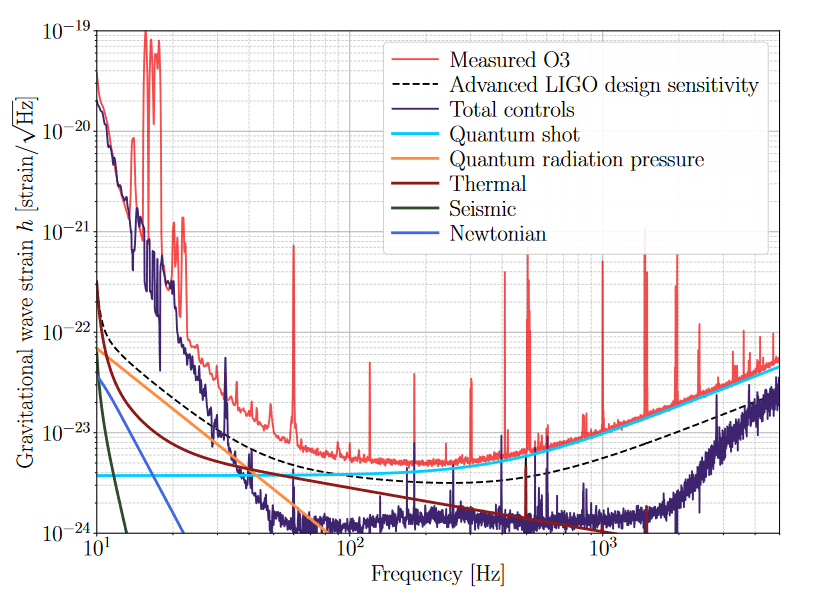
\includegraphics[width=\textwidth]{figures/basic_data_analysis/O3_noise_budget.PNG}
    \caption{O3 noise budget. Only few noise sources are shown for a simplified picture. \cite{aLIGO:2020wna}}
    \label{fig:O3_noise_budget}
\end{figure*}







\subsection{Basics of Fourier domain analysis}

Fourier domain analysis is a mathematical technique widely used in the field of data analysis to extract signal information from noisy data. Gravitational wave signals are often buried in noise, making it difficult to detect them in the time domain. However, by transforming the data into the frequency domain using Fourier analysis, it becomes easier to identify and analyze these signals.


Suppose we have a function of time $x(t)$. Let us denote the Fourier transform of $x(t)$ by $\tilde{x}(f)$, which is given by
    \begin{align}
        \tilde{x}(f) = \int_{-\infty}^{\infty} e^{-2\pi i ft} x(t) dt,
    \end{align}
    similarly, the inverse Fourier transform is given by
    \begin{align}
        x(t) = \int_{-\infty}^{\infty} e^{2\pi i f t} \tilde{x}(f) df.
    \end{align}

Write the discretized form of Fourier transform and talk about the Nyquist-frequency

\subsection{Modeling and measuring the noise}
The noise time series in a detector like LIGO is a complex superposition of various stochastic processes and we represent this time series $n(t)$ which can be considered as a vector $\textbf{n}$ (or random process). Each of the discrete samples $n_i = n(t_i)$ is described as random variable with values according a probability distribution $p_i = p(n_i)$, and the complete noise vector is then associated to to a joint probability distribution $p(\textbf{n})$. 

Features of the shape of a probability distribution can be captured by measuring moments. The first two moments of a stochastic process are often of particular interest -- mean $\mu = \langle \textbf{n}\rangle$ and covariance $C_{ij} = \langle(n-\mu_{i})(\mu_{j}-n)\rangle$, where $\langle\rangle$ is defined as the expectation value of a random variable over time. Assuming the noise process to be \textit{stationary random process} -- the statistical properties do not change over time. The ensemble average is equivalent to a long time average. We can estimate these two quantities from the data with $N$ data samples
\begin{align}
    \mu = \dfrac{1}{N}\sum_{i=1}^{N}n_{i}.
    \label{eq:mean-noise-series}
\end{align}
And, the covariance matrix can be estimated using
\begin{align}
    C_{ij} = (n_{i} - \mu)(\mu - n_j).
    \label{eq:covariance-noise-series}
\end{align}
We can write the joint probabilty distribution of noise $p(\textbf{n})$ in terms of the mean and the covariance matrix which follows a multi-variate normal distribution
\begin{align}
    p(\textbf{n}) = \dfrac{1}{\text{det}(2\pi \textbf{C})^{1/2}}\text{exp}\Bigg[-\dfrac{1}{2} \sum_{ij}(n_{i} - \mu)(\mu - n_j) C_{ij}^{-1} \Bigg],
    \label{eq:joint-pdf-noise}
\end{align}
where $C_{ij}^{-1}$ represents the inverse and $\det{C}$ the determinant of the covariance matrix.


\section{Optimal method to extract signal out of noise: Matched filtering}
At the heart of modeled approaches to detecting compact binary coalescence (CBC) signals lies the matched-filtering method. This technique scans through data from interferometers to identify patterns that match the predicted gravitational wave (GW) signal waveforms referenced in the literature. This section provides a succinct overview of matched filtering and highlights some innovative approaches to enhance the efficiency of these algorithms. Additionally, we reflect on past strategies that have aimed at optimizing matched filtering, as discussed in Section II B.

When it comes to GW signals emanating from CBC sources with circular orbits, they are described by 15 distinct parameters, as cited in studies. These parameters fall into two groups: (1) intrinsic parameters, which include the masses $(m_1, m_2)$ and three-dimensional spin vectors $(\chi_1, \chi_2)$, and (2) extrinsic parameters that are defined from the perspective of the observer—these are the standard spherical coordinates $(D, i, \psi)$, position in the sky $(\theta, \phi)$, and the coalescence timing and phase $(t_c; \phi_c)$. These parameters allow for the GW signal to be precisely depicted through a combination of analytical and numerical methods .

To detect the anticipated GW signal, denoted as $\tilde{h}(f)$ and commonly referred to as the template, one executes matched filtering in the frequency domain. This process assesses the probability that a set of data includes the specific template. The statistic used in matched filtering is essentially a correlation — it involves the Fourier-transformed data $[\tilde{s}(f)]$ and the template $[\tilde{h}(f)]$ — and takes into account the noise power spectral density (PSD) $S_n(f)$. It is established that the matched filter serves as the optimal statistical measure for signal detection amidst stationary Gaussian noise.

The mathematical expression for the complex matched filter statistic is:
\begin{align}
    \label{Eq:matched_filter}
    \braket{s|h} = 4\int_{0}^{\infty} \dfrac{\tilde{s}(f)\tilde{h}^*(f)}{S_n(f)}.
\end{align}
The signal-to-noise (SNR) ratio $\rho$ which is the matched-filter output maximised over an overall amplitude,   
\begin{align}
    \label{Eq:SNR_def}
    \rho^2 = \dfrac{(\Real[\braket{s|h}])^2}{\braket{h|h}}.
\end{align}

Since the signal parameters are unknown, the SNR is maximised over the parameter space. A naive maximisation procedure over the complete 15-dimensional parameter space is computationally challenging. Therefore, the component spins are typically assumed to be aligned with the orbital angular momentum and a search is conducted only for the dominant gravitational-wave mode. Under these assumptions the two polarizations of the signal are related by a simple phase shift $\tilde{h}_+(f) = i \tilde{h}_{\times}(f)$. Using Eqs.(\ref{Eq:Detector_response}) and (\ref{Eq:spherical_harmonics}) the signal seen by the detector in Fourier domain is simplified to 
\begin{align}
    \label{Eq:maxmising_templates}
    \tilde{h}(f) = A(f)e^{i \phi_0}\tilde{h}_0(\kappa; f)e^{2\pi i f t_c},
\end{align}
where $\tilde{h}_0(\kappa)$ depends only on the intrinsic parameters and the extrinsic parameters are factored out as the nuisance parameters -- an overall amplitude $A$ and phase $\phi_0$. 

As per Eq. (\ref{Eq:maxmising_templates}) the SNR is maximised in three categories of parameters -- 1) Intrisinc parameters $\kappa$, 2) fiducial parameters $A$ and $\phi_0$ 3) time of arrival $t_c$. The intrinsic parameters are searched by using a set of discrete points laid out on the four dimensional parameter space $\kappa^{||} = (m_1, m_2, \chi_{1z}, \chi_{2z})$. Waveforms evaluated with parameter values at a given sampled point is referred as templates and together they make up a template bank. The matched filter is repeatedly computed over all the templates to find the best matching template with highest SNR. Simultaneously, for each template, the SNR is maximised over the extrinsic parameters $(D, i, \psi, \alpha, \delta, \varphi_c)$ via the nuisance parameters ($A, \phi_0$) -- first by normalizing the matched filter with the power of the signal $\braket{h|h}$, and then using a quadrature of the SNR to maximise the unknown phase $\phi_0$. The maximization over these nuisance parameters is written as 
\begin{align}
    \mathop{\max}_{\phi_{0}}(\rho^2) = \dfrac{1}{2}\norm{\braket{s|\hat{h}_0}}^2,
    \label{Eq:simplified_statistics}
\end{align}
where $\hat{h}_0 = \tilde{h}_0/\braket{\tilde{h}_0|\tilde{h}_0}^{1/2}$. Finally, the position of the signal is efficiently searched over by performing an inverse fast Fourier transformation (FFT) to obtain the SNR time-series.

\section{Detection in non-Gaussian noise}

\section{}